\documentclass{article}
\usepackage[utf8]{inputenc}

\title{Theory and Applications of  Hadamard Matrices}
\author{Nicolas Bravo \\ nbravo@mit.edu }
\date{May 2015}

%\usepackage{natbib}
\usepackage{graphicx}
\usepackage{amsmath}
\usepackage{amsthm}

\newtheorem{theorem}{Theorem}[section]
\newtheorem{corollary}{Corollary}[theorem]
\newtheorem{lemma}{Lemma}[theorem]
\theoremstyle{definition}
\newtheorem{definition}{Definition}[section]

%\renewcommand\qedsymbol{$\blacksquare$}

\begin{document}

\maketitle

\section{Abstract}
This paper will discuss a number of interesting results regarding Hadamard matrices. We begin by giving some context about why Hadamard matrices might be useful and how mathematicians first became interested in them. The content in this paper is based primarily on Chapter 7 of \emph{Proofs from the Book}\cite{pftb}

\section{Introduction}
In the late 1800s, French mathematician Jacques Hadamard began investigating a question regarding matrix determinants. If we consider the set of real square matrices $A = (a_{ij})$ with $|a_{ij}| \leq 1$, what is $\underset{A}{\max} \det A$? He eventually discovered a bound for the determinants of such matrices:
$$ |\det A| \leq \sqrt{n^n} $$
with equality when the entries of $A$ are exactly $\pm 1$ and the rows of $A$ are pairwise orthogonal. Matrices that satisfy both of these requirements are defined to be Hadamard matrices.

\begin{definition}
 A Hadamard matrix is a square matrix whose entries are either +1 or -1 and whose rows are mutually orthogonal.
\end{definition}

At this point we should prove the bound on $|\det A|$ and show why Hadamard matrices attain the maximum value.
\begin{theorem}
Let $A$  be an $n \times n$ real matrix whose entries satisfy $| a_{ij} | \leq 1$ for all $i , j$.  Then $| \det ( A) | \leq n^{\frac n  2}$ .  Equality holds if and only if $A$ is a Hadamard matrix.
\end{theorem}

\begin{proof}
 We'll take a geometric approach to this proof. Let the rows of $A$ be $a_1, a_2, \ldots, a_n$. Then we can interpret $|\det(A)|$ as the volume of a parallelipiped with sides $a_1, \ldots, a_n$. Therefore,
 $$ |\det(A)| \leq |a_1||a_2| \ldots |a_n|$$
 where equality holds only if and only if all sides (rows of $A$ are perpendicular). We also know that
 \begin{align*}
 |a_i| &= \left( \sum_{j = 1}^n a_{ij}^2 \right)^{\frac 1 2} \\
 & \leq \sqrt n
 \end{align*}
 where equality in this case holds if and only if $|x_{ij}| = 1$ for all $j$. Therefore  $| \det ( A) | = n^{\frac n  2}$ if and only if $A$ is a matrix with entries $\pm 1$ and all rows mutually orthogonal, which makes $A$ a Hadamard matrix.
\end{proof}


\section{Existence and Construction}
One of the most important questions regarding Hadamard matrices is the following: for which $n$ does an $n \times n$ Hadamard matrix exist?. We certainly know that, for example, there cannot be any Hadamard matrices with odd $n$ since the rows could not possibly be orthogonal to each other. On the other hand, we can systematically construct Hadamard matrices for certain values of $n$.

The following construction, know as Sylvester's construction \cite{construction}, gives us Hadamard matrices for all $n = 2^k$. Let $H$ be a Hadamard matrix of order $n$. Then
\begin{equation*}
\begin{bmatrix}
H & H \\
H & -H
\end{bmatrix}
\end{equation*}
is a Hadamard matrix of order $2n$. This construction could lead to the following sequence of Hadamard matrices:
$H_1 =
\begin{bmatrix}
1
\end{bmatrix},
$
$H_2 =
\begin{bmatrix}
1 & 1 \\
1 & -1 \\
\end{bmatrix},
$
$H_{2^k} =
\begin{bmatrix}
H_{2^{k-1}} & H_{2^{k-1}} \\
H_{2^{k-1}} & -H_{2^{k-1}}
\end{bmatrix}
$
This gives us Hadamard matrices for all powers of 2. Alternatively, Paley's construction can give us Hadamard matrices of order $q +1$ where $q$ is a prime number congruent to $3 \mod 4$. In other words, Paley's construction can give us Hadamard matrices of order 12, 20, 24, and so on.  A generalization of Sylvester's construction proves that if $H_n$ and $H_m$ are Hadamard matrices of orders $n$ and $m$ respectively, then $H_n \otimes H_m$ is a Hadamard matrix of order $nm$.

There is a conjecture which proposes that a Hadamard matrix of order $4k$ exists for every positive integer $k$. Although unproven, it is widely regarded as highly likely to be true. As of 2008, there are only 13 multiples of 4 less than or equal to 2000 for which no Hadamard matrix of that order is known. They are: 668, 716, 892, 1004, 1132, 1244, 1388, 1436, 1676, 1772, 1916, 1948, and 1964 \cite{existence}.

Although it is unknown whether a Hadamard matrix of order $4k$ exists for every $k$, it \emph{is} known that if a Hadamard matrix exists for order $n$ then $n$ can be one of only a limited set of values:
\begin{theorem}
If $H$ is an $n \times n$ Hadamard matrix, then $n = 1$ or $n = 2$ or $n \equiv 0 \mod 4$.
\end{theorem}

\begin{proof}
We know that Hadamard matrices exist for $n=1$ and $n=2$ by construction. We also know that $n$ must be even because the orthogonality of the rows implies that there are exactly as many $+1$ entries as there are $-1$ entries in each row. All that remains is to show that for $n > 3$, $4|n$.\\

First, we know that we can negate an entire column in a Hadamard matrix and the result will also be Hadamard. Therefore we can selectively multiply columns in $H$ until the first row consists entirely of 1's. Then for each column there are exactly 4 possibilities for the first 3 entries in that column: $+++, ++-, +-+,$ or $+--$. Let's say that each possibility occurs $a, b, c,$ and $d$ times respectively. If we take advantage of the orthogonality relations on these first three rows we obtain the following set of equations:
\begin{align*}
  a + b + c + d &= n\\
  a + b - c - d &= 0\\
  a - b + c - d &= 0\\
  a - b - c + d &= 0
\end{align*}
If we add all of these equations we obtain $4a = n$, thus proving that $n$ must be a multiple of 4.
\end{proof}

\section{Equivalence of Hadamard Matrices}
In the previous proof we briefly mentioned that we can negate a column of a Hadamard matrix and the result will still be Hadamard.
In fact, given a Hadamard matrix $H$, we can perform a number of interesting operations on $H$ and still end up with a Hadamard matrix. In particular, we can perform any of the following operations any number of times:
\begin{itemize}
  \item Interchange any two rows or any two columns
  \item Multiply any row or any column by -1
  \item Transpose
\end{itemize}
and the result will still be Hadamard. If we can transform $H$ into $H'$ through a sequence of the above operations then we say that $H$ and $H'$ are equivalent. The problem of determining whether two Hadamard matrices are equivalent turns out to be very difficult; the interested reader is highly encouraged to look into the topic on his own.\\

For a given order $n$ there may be only one distinct (i.e. non-equivalent) Hadamard matrix or there may be several. The table below gives the number of distict Hadamard matrices for various orders \cite{orders}.
\begin{figure}[h!]
\caption{Number of distinct Hadamard matrices for various orders}
\centering
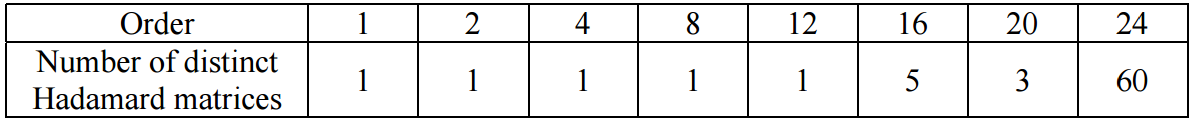
\includegraphics[width=1.3\textwidth]{table}
\end{figure}

\section{Nearly Hadamard Matrices}
Although it is conjectured that there is a Hadamard matrix for every order that is a multiple of 4, the results we have shown so far do not apply unless we can actually find those matrices. For example, when $n=668$ we do not know for sure whether there is an $n \times n$ matrix $A$ where each entry is between 1 and -1 and whose determinant achieves the maximum theoretical bound of $\sqrt {n^n}$. However, for $n$ not divisible by 4 we would still like to see if we can find a lower bound for $\underset{A}{\max |\det A|}$. The following theorem gives us such a lower bound for square matrices with entries $\pm 1$. These matrices are in a sense similar to Hadamard matrices although they do not necessarily have all rows mutually orthogonal. For this reason we may like to think of them as ``nearly Hadamard".

\begin{theorem}
There exists an $n \times n$ matrix with entries $\pm 1$ whose determinant is greater than $\sqrt{n!}$
\end{theorem}

\begin{proof}
We begin by considering the root mean square of all $2^{n^2}$ matrices with $\pm 1$ entries. Then we have
$$ D_n = \frac{\sqrt{\sum_A (\text{det } A)^2}}{2^{n^2}}$$
and it should be clear that
$$ \underset{A}{\max} |\det| A \geq D_n$$
so our goal is to obtain a bound on $D_n$.\\

The idea will be to use the definition of the determinant to write out the sum $\sum_A (\det A)^2$ and interchange the appropriate summations in such a way that the terms simplify nicely.

Recall that we define the determinant of a matrix $A$ as
$$ \det(A) = \sum_{\sigma \in S_n} \text{sign}(\sigma) \prod_{i=1}^n a_{i, \sigma_i}$$
where $\sigma$ is a permutation of the set $\{1,2,\ldots,n\}$ and $\text{sign}(\sigma)$ takes a value of $\pm 1$ depending on the permutation $\sigma$. We can then write

\begin{align*}
  D_n^2 &= \frac{1}{2^{n^2}} \sum_A \left(\sum_{\pi} \text{sign}(\pi) \prod_{i=1}^n a_{i,\pi_i}\right)^2\\
  &= \frac{1}{2^{n^2}} \sum_A \sum_{\sigma} \sum_{\tau} \text{sign}(\sigma) \text{sign}(\tau) \prod_{i=1}^n a_{i,\sigma_i} a_{i,\tau_i}\\
\end{align*}

In this last expression, the inner two sums compute the square of the determinant for each matrix while the outer sum sums over all matrices. We will exchange the order of summations so that instead, we consider pairs of permutations $\sigma$ and $\tau$ in the outer sum and for each pair we sum over each matrix $A$ in the inner sum. In other words, we rewrite as
$$
  D_n^2 = \frac{1}{2^{n^2}} \sum_{\sigma, \tau}\text{sign}(\sigma) \text{sign}(\tau) \left(\sum_A \prod_{i=1}^n a_{i,\sigma_i}  a_{i,\tau_i} \right)\\
  $$

  Now we will rewrite the inner sum once more. Specifically, note that since we are considering all matrices $A$ with entries $\pm 1$, summing over all $A$ is equivalent to summing over $\sum_{a_{11} = \pm 1} \sum_{a_{12} = \pm 1} \dots \sum_{a_{nn} = \pm 1}$

  So we rewrite the inner sum as $\sum_{a_{11} = \pm 1} \sum_{a_{12} = \pm 1} \dots \sum_{a_{nn} = \pm 1} \prod_{i=1}^n a_{i,\sigma_i}  a_{i,\tau_i}$.

  The most important thing about this sum is that it is 0 when $\sigma \neq \tau$. When $\sigma = \tau$, however, the inner product evaluates to 1 and so we have
  $$ \sum_{a_{11} = \pm 1} \sum_{a_{12} = \pm 1} \dots \sum_{a_{nn} = \pm 1} 1 = 2^{n^2}$$
  So we can finally rewrite our original expression as
  \begin{align*}
  D_n^2 &= \frac{1}{2^{n^2}} \sum_{\sigma} 2^{n^2} \\
  &= n!\\
  D_n &= \sqrt{n!}
  \end{align*}

  And we conclude that $\underset{A}{\max} \det A \geq \sqrt n!$
\end{proof}

\section{Applications}
Many applications of Hadamard matrices become more apparent when we look at their definition in a slightly different way. Throughout this paper we have been discussing matrices with entries $\pm 1$, but we can extend the idea to include binary-valued matrices in general, such as matrices with all entries 0 or 1. Similarly, the requirement of orthogonal rows can be thought of as a simple requirement than any two rows must differ in exactly $\frac n 2$ places.

With that in mind, Hadamard matrices find surprising useful applications in coding theory. In particular, they are useful in finding error-correcting codes. Error-correcting codes are used to send messages reliably over unreliable channels. If we know that there is a Hadamard matrix of order $n$ then we know there is a binary code with $2n$ code words and a minimum distance of $\frac n 2$ between code words \cite{applications}. Without going too much into coding theory, we will state that a minimum distance of $\frac n 2$ between code words is significant because it allows for maximal error correcting capability for a code word of length $n$.


\section{Conclusion}
We have shown that Hadamard matrices are special because their determinant achieves the maximum possible value for a real square matrix withentries in the range $[-1,1]$, which is  $n^{\frac{n}{2}}$. It is known that all Hadamard matrices must have order 1,2, or a multiple of 4, and it is conjectured that at least one exists for every multiple of 4. When the upper bound of $n^{\frac n 2}$ cannot be achieved by a Hadamard matrix, we can still place a lower bound on $\max \det A$ if $A$ is ``nearly Hadamard".

\newpage
\begin{thebibliography}{1}

  \bibitem{pftb} Aigner, Martin, and Gunter M. Ziegler. "The Spectral Theorem and Hadamard's Determinant Problem." \emph{Proofs from the Book. Berlin: Springer, 2004. N. pag. Print.}

  \bibitem{applications} J. Seberry, B. J. Wysocki, and T. A. Wysocki. "On some applications of Hadamard matrices" \emph{Faculty of Informatics - Papers} (2005).

  \bibitem{construction} Cameron, Peter J. "Hadamard Matrices." \emph{Encyclopedia of Statistical Sciences} (2004): n. pag. \emph{Designtheory.org}. 8 June 2006. Web. 10 May 2015. <http://designtheory.org/library/encyc/topics/had.pdf>.

  \bibitem{orders} Wentink, Allan. "Hadamard Matrices and Designs." \emph{Combinatorial Designs} (2004): 73-100. Cs.arizona.edu. 2004. Web. 10 May 2015. <https://www.cs.arizona.edu/patterns/weaving/webdocs/wa\_hadmtx.pdf>.

  \bibitem{existence} Dokovic, Dragomir Z (2008). "Hadamard matrices of order 764 exist". \emph{Combinatorica} 28 (4): 487–489.

\end{thebibliography}

\end{document}

